\section{Results}
\label{sec:results}

\todo[inline]{should I evaluate with direct lighting integrator or path? direct lighting would show the resutls more clearly, but ideally I show results for actual rendering right? Also could do both of course, what do you think?}

We evaluate the method presented for a scene containing a variety of lights each with their corresponding portals. We compare portal sampling, using antishadow volumes to set the portal sampling distributions. The reference image was produced using an unbiased unidirectional path tracer, using light sampling, and $x$ samples per pixel. We then compare the mean squared error over time of portal sampling and light sampling.

\begin{figure*}[ht]
    \centering
    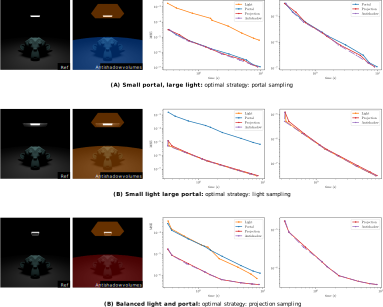
\includegraphics[width=0.95\textwidth]{results.png}
    \caption{{\color{red} Image is a bit sketchy (and data is fake), but feedback on the composition might be useful} We compare the convergence rates for light sampling (Light) and portal sampling (Portal). The listed errors are for the highlighted image insets. As seen, portal sampling is the most robust method, regardless of the size ratio between the light and the portal}
    \label{fig:fake-results}
\end{figure*}